\documentclass[a4paper]{article}
\usepackage[utf8]{inputenc}
\usepackage[IL2]{fontenc}
\usepackage[czech]{babel}
\usepackage{amsmath}
\usepackage{fullpage}
\usepackage[pdftex]{graphicx}
\usepackage[font=small,format=plain,labelfont=bf,up,textfont=it,up]{caption}
\usepackage[final]{pdfpages}
\usepackage{pdflscape}

\usepackage[pdftex,unicode,hidelinks]{hyperref}

\title{Lambert CZ -- nové zobrazení pro Česko}
\date{\today}
\author{Jan Šimbera}

\newcommand{\file}[1]{\texttt{#1}}
\newcommand{\term}[1]{\emph{#1}}
\newcommand{\dg}{^{\circ}}

\hyphenation{kom-pro-mis}

\begin{document}
\maketitle
\begin{abstract}
V současnosti nejvíce rozšířené kartografické zobrazení pro Česko je Křovákovo zobrazení, které ale z mnoha ohledů nevyhovuje pro současnou GIS a kartografickou praxi. Tento dokument představuje alternativu založenou na Lambertově úhlojevném kuželovém zobrazení.
\end{abstract}

\section{Popis zobrazení}
Zobrazení je variantou Lambertova sečného úhlojevného \emph{(konformního)} kuželového zobrazení z elipsoidu do roviny v normální poloze. Počítá s využitím evropského referenčního elipsoidu ETRS89. 

\subsection{Parametry zobrazení}
Parametry jsou následující:
\begin{itemize}
  \item orientace os: standardní matematická
  \item poloha kužele: normální (kartografický pól totožný se severním zeměpisným)
  \item základní poledník $\lambda_0 = 15\dg$
  \item základní rovnoběžka $\varphi_0 = 49\dg 45'$
  \item sečné rovnoběžky:
    \begin{itemize}
      \item $\varphi_1 = 49\dg$
      \item $\varphi_2 = 50\dg 30'$
    \end{itemize}
  \item posun ve směru osy x \emph{(false easting)} $\Delta x = 250\,000$ m
  \item posun ve směru osy y \emph{(false northing)} $\Delta y = 150\,000$ m
\end{itemize}

\subsection{Definice ve WKT}
Definiční WKT soubor má tvar:
\begin{verbatim}
PROJCS["Lambert_CZ",
  GEOGCS["GCS_ETRS_1989",
    DATUM["D_ETRS_1989",SPHEROID["GRS_1980",6378137.0,298.257222101]],
    PRIMEM["Greenwich",0.0],
    UNIT["Degree",0.0174532925199433]
  ],
  PROJECTION["Lambert_Conformal_Conic"],
  PARAMETER["False_Easting",250000.0],
  PARAMETER["False_Northing",150000.0],
  PARAMETER["Central_Meridian",15.0],
  PARAMETER["Standard_Parallel_1",49.0],
  PARAMETER["Standard_Parallel_2",50.5],
  PARAMETER["Scale_Factor",1.0],
  PARAMETER["Latitude_Of_Origin",49.75],
  UNIT["Meter",1.0]
]
\end{verbatim}

\subsection{Definice v Proj4}
Definice ve formátu pro Proj4 má tvar:
\begin{verbatim}
+proj=lcc +lat_1=49 +lat_2=50.5 +lat_0=49.75 +lon_0=15 +x_0=250000 +y_0=150000
+ellps=GRS80 +towgs84=0,0,0,0,0,0,0 +units=m +no_defs
\end{verbatim}

\subsection{Zdůvodnění}
Souřadnicový systém ETRS89 je použit z důvodu snadné návaznosti na mapování na evropské a světové úrovni -- jeho souřadnice jsou jednoduše převoditelné do elipsoidu WGS84. Díky navázání na evropskou tektonickou desku se také nebudou v čase měnit kontinentálním driftem. Podkladový elipsoid GRS80 je velmi přesný a v současnosti nejčastěji používaný. ETRS89 neobsahuje chyby akumulované při tvorbě systému S-JTSK.

Kuželové zobrazení v normální poloze je vhodné pro území protažená v rovnoběžkovém směru, tedy i Česko. Obecnou polohu kužele, kterou používá zobrazení Křovákovo, je možno díky neuvažování Slovenska bez většího nárůstu zkreslení opustit.

Úhlojevné zobrazení je zvoleno kvůli návaznosti na existující systém; zachovaná vysoká přesnost v kombinaci s touto vlastností umožňuje i geodetické aplikace, a tedy výhledově úplné opuštění S-JTSK. Zkreslení ploch je díky malé velikosti mapovaného území stále zcela v mezích současných standardů (viz příslušná sekce).

Parametry zobrazení byly zvoleny na základě numerické optimalizace zkreslení a následně zaokrouhleny:
\begin{itemize}
\item Základní poledník 15$\dg$ je porovnatelný s UTM, běžně používaný a z celočíselných poledníků nejblíže středu území.
\item Základní rovnoběžka a sečné rovnoběžky jsou zvoleny v souladu s pravidly pro minimalizaci zkreslení a jsou velmi blízké minimálním dosažitelným hodnotám.
\item Posuny souřadnic (false northing a easting) jsou zvoleny jako vhodná kulatá čísla tak, aby hodnoty souřadnic byly na celém území Česka kladné a přitom nepříliš vysoké.
\end{itemize}

\subsection{Zobrazovací rovnice}
\subsubsection{Konstanty zobrazení}
\begin{align*}
q = a \frac{w(\varphi_1)}{n t(\varphi_1)^n} &= 11\,583\,124,653\,549\,\mathrm{m}\\
n = \frac{\ln{w(\varphi_1)} - \ln{w(\varphi_2)}}{\ln{t(\varphi_1)} - \ln{t(\varphi_2)}} &= 0,766\,083\,775\,796\\
\rho_0 = \rho(\varphi_0) &= 5\,361\,345,963\,200\,\mathrm{m},
\end{align*}
kde $w$ je poměr
\begin{equation*}
w(\varphi) = \frac{\cos{\varphi}}{\sqrt{1 - e^2 \sin^2{\varphi}}} = \frac{N(\varphi) \cos{\varphi}}{a},
\end{equation*}
$a$ a $e$ parametry elipsoidu GRS80
\begin{align*}
a &= 6\,378\,137\,\mathrm{m}\\
e &= 0,006\,694\,380
\end{align*}
a parametry $t$ a $\rho$
\begin{align*}
\rho(\varphi) &= q t(\varphi)^n\\
t(\varphi) &= \tan{\left(\frac{\pi}{4} - \frac{\varphi}{2}\right)}\left(\frac{1+e\sin{\varphi}}{1-e\sin{\varphi}}\right)^{\frac{e}{2}}
\end{align*}

\subsubsection{Přímá transformace}
Zobrazovací rovnice pro převod z geografických souřadnic na pravoúhlé mají tvar:
\begin{align*}
x &= \rho \sin{\theta} + \Delta x\\
y &= \rho_0 - \rho \cos{\theta} + \Delta y,
\end{align*}
kde
\begin{equation*}
\theta(\lambda) = n (\lambda - \lambda_0).
\end{equation*}
  
\subsubsection{Inverzní transformace}
Zeměpisná délka se z pravoúhlých souřadnic získá přímým vztahem
\begin{equation*}
\lambda = \frac{1}{n} \arctan{\frac{x - \Delta x}{\rho_0 - (y - \Delta y)}}.
\end{equation*}
Zeměpisnou šířku je třeba spočítat iterativně. Počáteční odhad je
\begin{equation*}
\varphi_{(1)} = \frac{\pi}{2} - 2 \arctan{\tau(x,y)},
\end{equation*}
kde
\begin{equation*}
\tau(x,y) = \left[\frac{1}{q}\sqrt{(x - \Delta x)^2 + [\rho_0 - (y - \Delta y)]^2}\right]^{\frac{1}{n}}.
\end{equation*}
Iterační výpočet má tvar
\begin{equation*}
\varphi_{(n+1)} = \frac{\pi}{2} - 2 \arctan{\left[\tau(x,y) \cdot \left(\frac{1-e\sin{\varphi_{(n)}}}{1+e\sin{\varphi_{(n)}}}\right)^{\frac{e}{2}}\right]},
\end{equation*}
pro konvergenci stačí zpravidla tři až čtyři iterace.

\section{Zdůvodnění a diskuze}
Takto navržené zobrazení má oproti Křovákovu zobrazení následující výhody:
\begin{itemize}
  \item Používá standardní elipsoid, v jehož souřadnicích je uváděna většina současných prostorových dat. Existuje pro něj globální transformační klíč bez nutnosti používat mezielipsoidické transformace a grid shift.
  \item Používá konvenční orientaci os, která nečiní problémy GIS softwaru. Hodnoty obou souřadnic jsou na celém území státu kladné.
  \item Je výpočetně méně náročné než Křovákovo zobrazení, neboť díky své přímé povaze a normální poloze používá pouze jeden krok.
  \item Všechny prvky zobrazení jsou již implementovány ve všech běžných GIS softwarech. 
  \item Hodnoty zkreslení jsou pro většinu území stejné jako u Křovákova zobrazení.
  \item Meridiánová konvergence je nižší a rovnoměrně rozložená kolem nuly, takže není třeba mapu celé republiky natáčet pro nezkreslené vnímání severního směru.
\end{itemize}

\subsection{Zkreslení}
Zkreslení délek v zobrazení je možno snadno určit pomocí vzorce pro měřítko délek
\begin{equation*}
m = \frac{n\rho}{N \cos{\varphi}} = \frac{n\rho(\varphi) \sqrt{1 - e^2 \sin^2{\varphi}}}{a \cos{\varphi}}
\end{equation*}
Díky konformitě je zkreslení nezávislé na směru; ze vzorce výše vyplývá, že je konstantní pro danou zeměpisnou šířku. Měřítko ploch je $P = m^2$.

Pro dané hodnoty nezkreslených rovnoběžek je zkreslení délek na celém území maximálně 17,5 cm/km a průměrně 5,7 cm/km. Optimální hodnoty průměrného zkreslení 3,56 cm/km lze dosáhnout při dvojici nezkreslených rovnoběžek 49,33$\dg$ a 50,16$\dg$ (maximální zkreslení 23,7 cm/km), optimální hodnoty maximálního zkreslení 11,94 cm/km při dvojici 48,92$\dg$ a 50,69$\dg$ (průměrné zkreslení 8,1 cm/km). Zvolenou dvojici lze tedy považovat za~kompromis mezi oběma cíli, navíc při zachování snadno zapamatovatelných hodnot.

\subsection{Mapa}
Obraz Česka se zeměpisnou sítí v tomto zobrazení je uveden na obrázku níže.

% \begin{landscape}
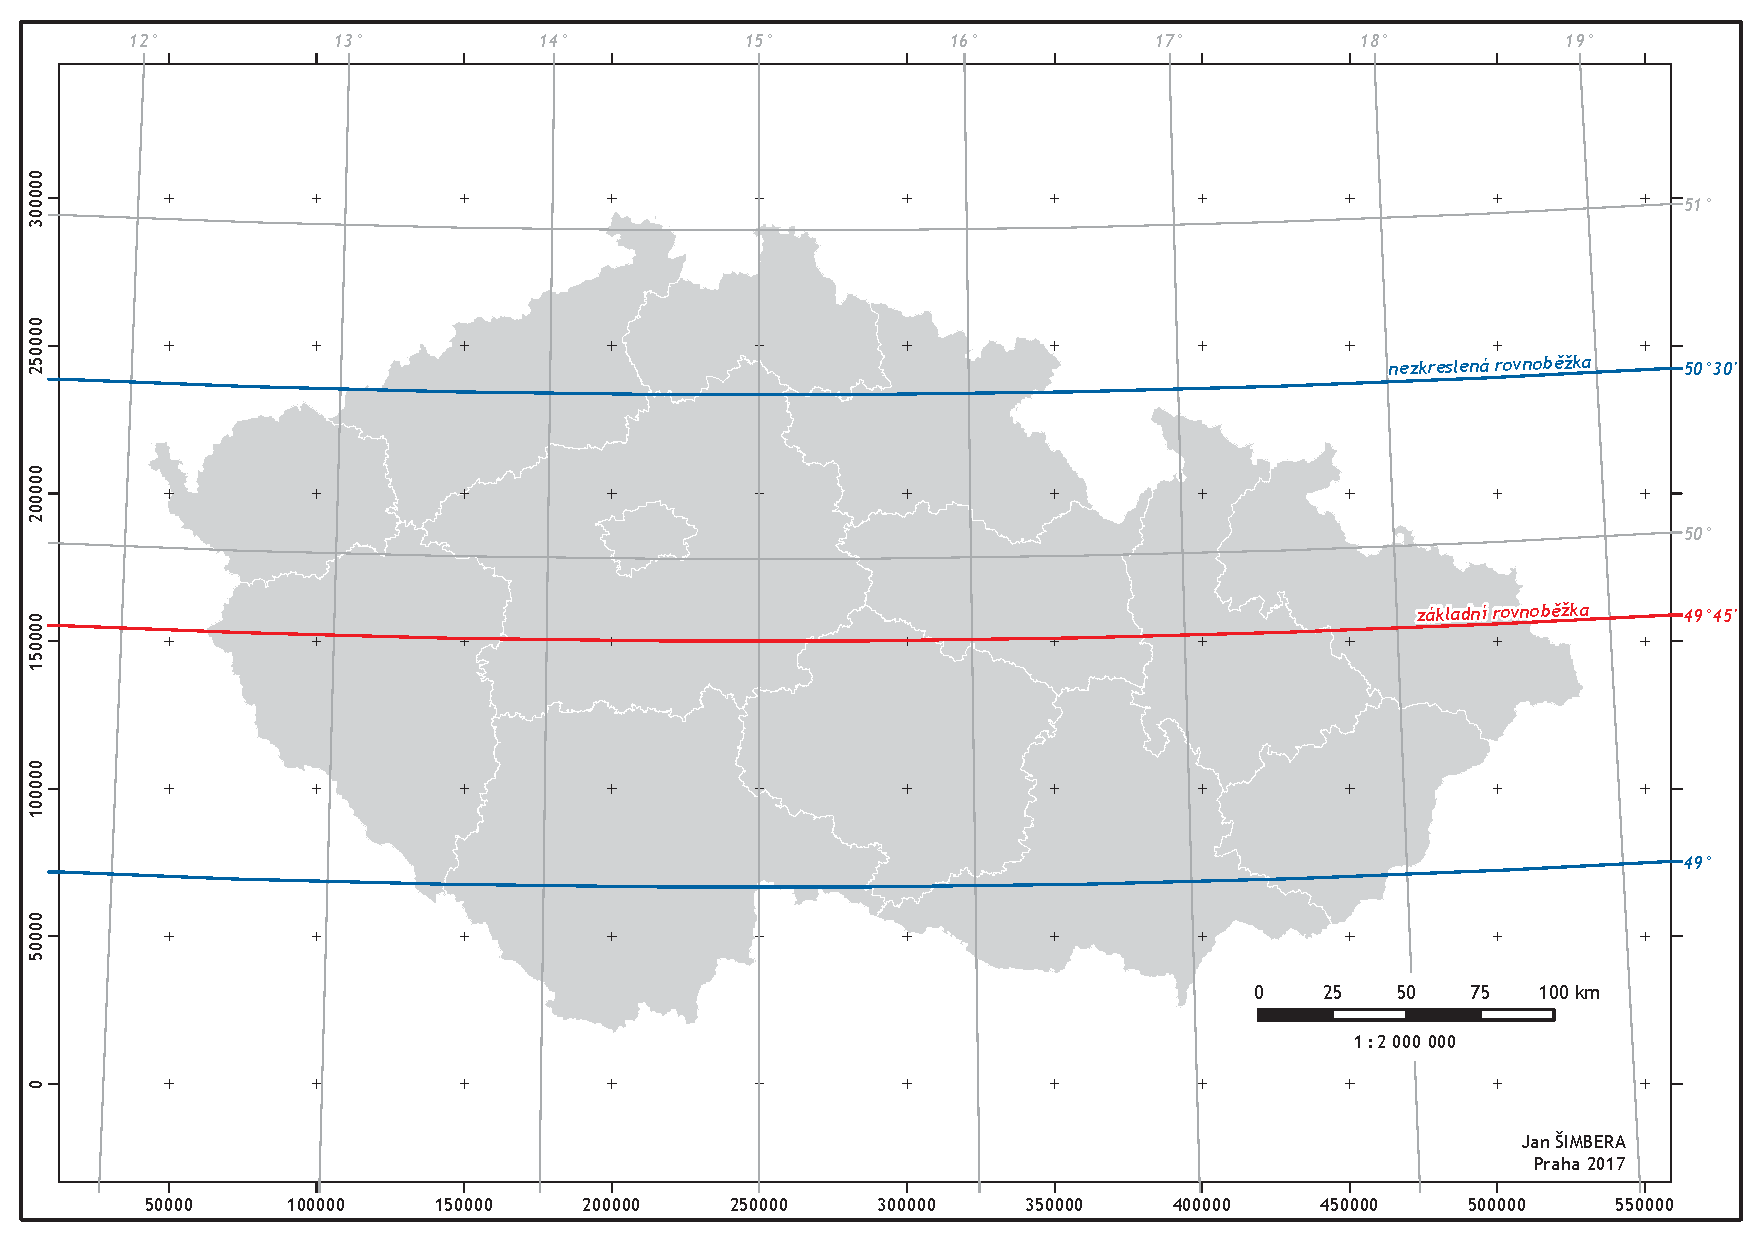
\includepdf[landscape=true]{map.pdf}
% \begin{figure}
% \centering
% \makebox[\textwidth]{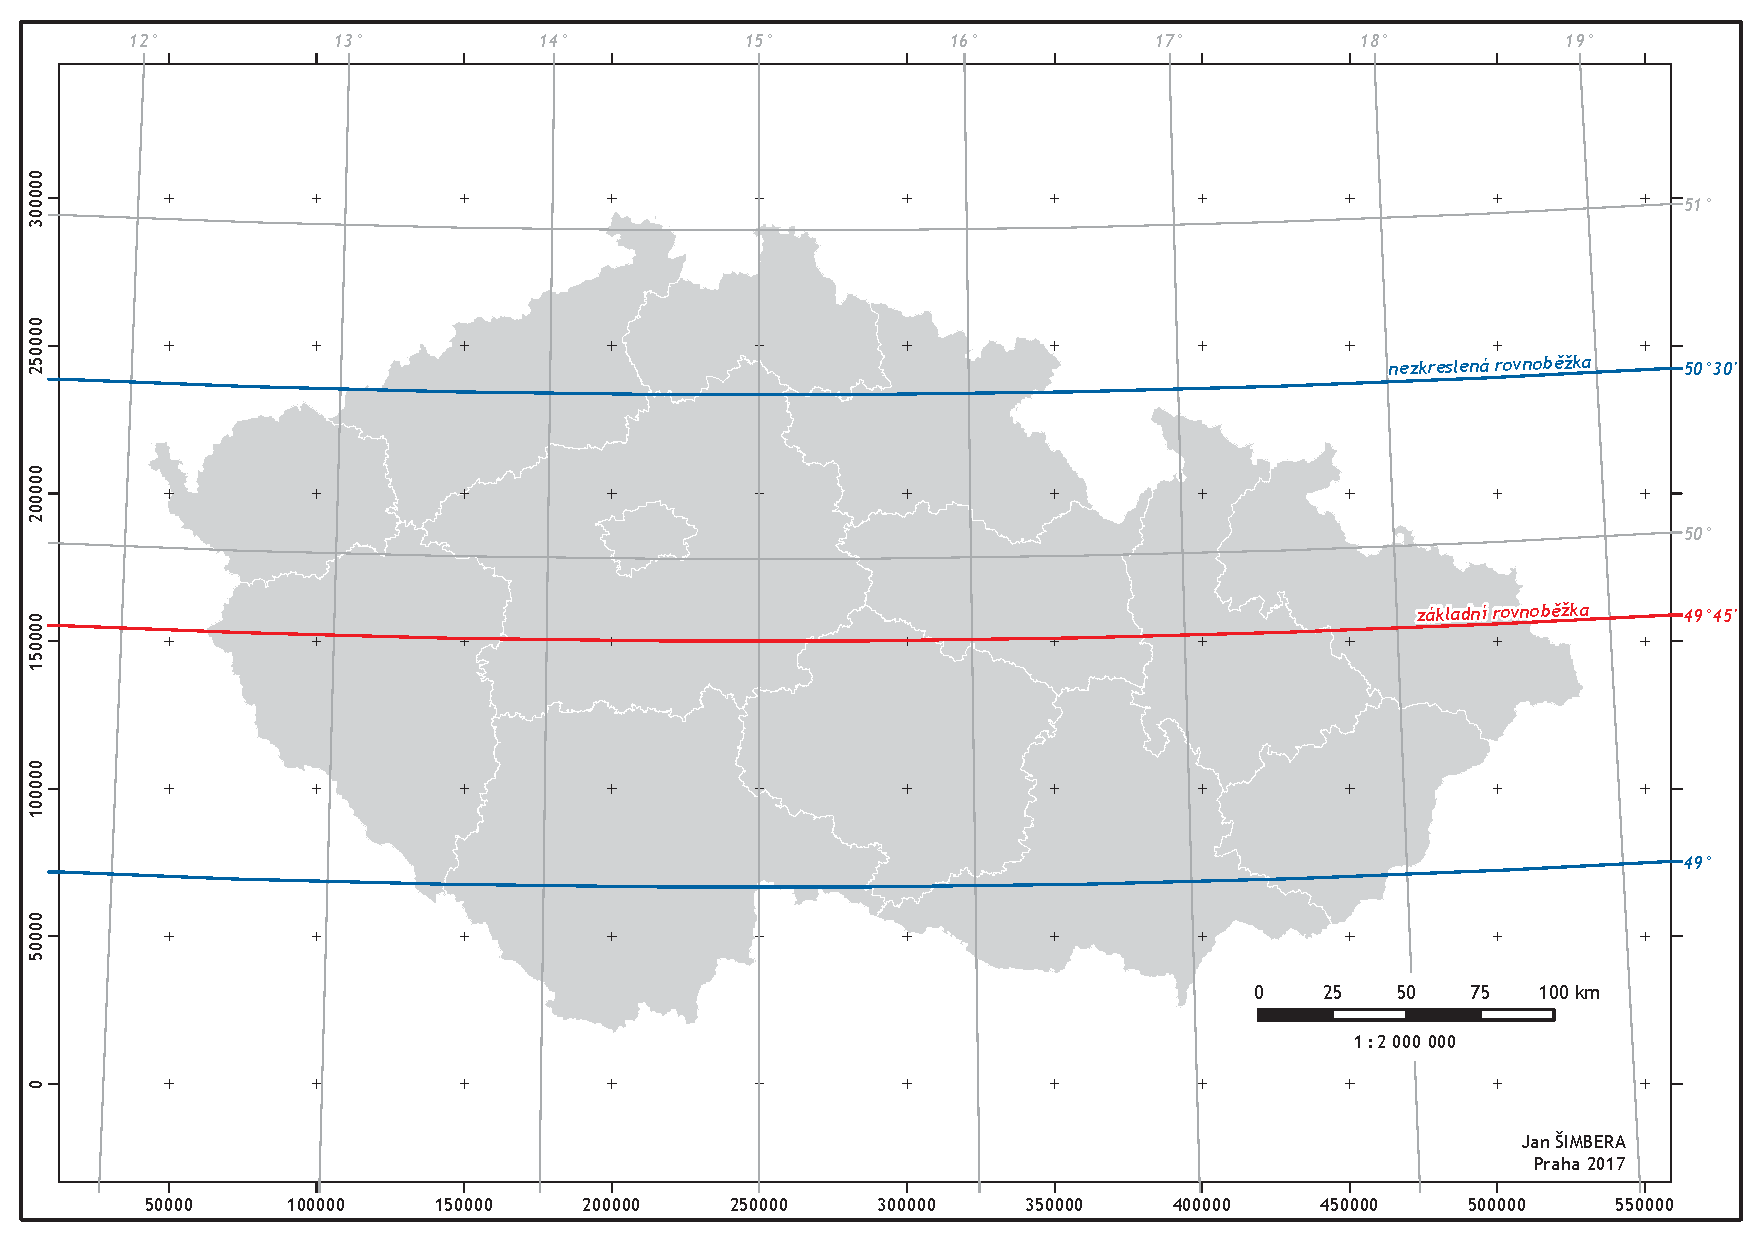
\includegraphics[width=1.5\textwidth]{map.pdf}}
% \end{figure}
% \end{landscape}
\end{document}